\documentclass[12pt]{article}
\usepackage{mathtext}
\usepackage{amsmath}
\usepackage[T2A]{fontenc}
\usepackage[utf8]{inputenc}
\usepackage[russian]{babel}
\usepackage[left=1.5cm, right=1.5cm, top=2cm, bottom=2cm, bindingoffset=0cm]{geometry}
\usepackage{listings}
\usepackage{fancyhdr}
\usepackage{pgfplots}
\pgfplotsset{compat=1.9}



\begin{document}
    \begin{center}
        \textbf{Московский авиационный институт} \\
        \textbf{(Национальный исследовательский университет)}
    \end{center} 
    ~\\
    ~\\
    Институт: «Информационные технологии и прикладная математика» \\
    Кафедра: 805 «Математическая кибернетика»  \\
    Дисциплина: «Численные методы»  
    ~\\
    ~\\
    ~\\
    \begin{center}
        Лабораторная работа №2 \\
        Тема: Решение начально-краевой задачи для дифференциального\\ уравнения 
        гиперболического типа
    \end{center}
    ~\\
    ~\\
    ~\\
    ~\\
    ~\\
    ~\\
    ~\\
    ~\\
    ~\\
    \begin{flushright}
        Студент: ~~~~~~~~~~~~Хахин Максим~~~~~~\\
        Группа: ~~~~~~~~~~~~~~80-403~~~~~~~~~~~~~~~~~\\
        Преподаватель: ~~~~Иванов И. Э.~~~~~~~\\
        Дата: ~~~~~~~~~~~~~~~~~~~~~~~~~~~~~~~~~~~~~~~~~~~\\
        Оценка: ~~~~~~~~~~~~~~~~~~~~~~~~~~~~~~~~~~~~~~~~\\
    \end{flushright}
    ~\\
    ~\\
    ~\\
    ~\\
    ~\\
    ~\\
    ~\\
    ~\\
    ~\\
    ~\\
    ~\\
    ~\\
    ~\\
    ~\\
    ~\\
    \begin{center}
        Москва, 2021
    \end{center}
    \pagestyle{empty}
    \newpage

    \pagestyle{fancy} 
        \fancyhead{}
        \fancyhead[L]{Хахин Максим}
        \fancyhead[R]{М8О-403Б-18} 
    \fancyfoot{} 
    \begin{enumerate}
        \item \textbf{Задание:}\\
        Используя явную схему крест и неявную схему, решить начально-краевую задачу для дифференциального уравнения гиперболического 
        типа. Аппроксимацию второго начального условия произвести с первым 
        и со вторым порядком. Осуществить реализацию трех вариантов 
        аппроксимации граничных условий, содержащих производные: 
        двухточечная аппроксимация с первым
        порядком, трехточечная аппроксимация со вторым порядком, 
        двухточечная аппроксимация со вторым порядком. В различные моменты 
        времени вычислить погрешность численного решения путем сравнения 
        результатов с приведенным в задании аналитическим решением. 
        Исследовать зависимость погрешности от сеточных параметров.
        \item \textbf{Вариант 9:}\\
        \begin{figure}[h]
            \center{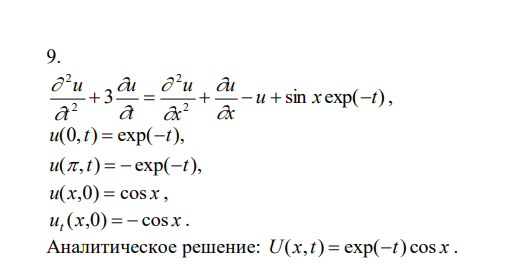
\includegraphics[width=0.5\linewidth]{ 1.png}}
            \label{ris:image}
        \end{figure}\\
        \item \textbf{Теория:}\\
        \begin{center}  \textbf{Разложение ДУ в ряд.} \end{center}
    Диференциальное уравнение с частными производными параболического типа в общем виде записывается следующим образом: 
    $$\frac{\delta^2 u}{\delta t^2}+ d\frac{\delta u}{\delta t}=a\frac{\delta^2 u}{\delta x^2}+b\frac{\delta u}{\delta x}+cu+f(x,t)$$
    \begin{enumerate}
    \item Для явной разностной схемы.
        \\Воспользуемся методами численного диференциирования и разложим каждый член уравнения имеющий производную в конечную сумму:
        \begin{itemize}
            \item $\frac{\delta^2 u}{\delta t^2} = \frac{u_{i}^{k-1}-2u_{i}^k+u_{i}^{k+1}}{\tau^2}$, где  $\tau$ - шаг по временной сетке;
            \item $d\frac{\delta u}{\delta t}=d\frac{u_i^{k+1}-u_i^{k-1}}{2\tau}$
            \item $a\frac{\delta^2 u}{\delta x^2} = a\frac{u_{i-1}^k-2u_{i}^k+u_{i+1}^k}{h^2}$, где  $h$ - шаг по пространственной сетке;
            \item $b\frac{\delta u}{\delta x} = b\frac{u_{i+1}^k-u_{i-1}^k}{2h}$;
            \item $cu = cu_{i}^k$;
        \end{itemize}
        Переппишем исходное уравнение:
        $$\frac{u_{i}^{k-1}-2u_{i}^k+u_{i}^{k+1}}{\tau^2}+d\frac{u_i^{k+1}-u_i^{k-1}}{2\tau} =a\frac{u_{i-1}^k-
        2u_{i}^k+u_{i+1}^k}{h^2}+b\frac{u_{i+1}^k-u_{i-1}^k}{2h}+cu_{i}^k+f(x,t).$$
        Сгруппируем коэффицениты при u с одинаковыми индексами:
        $$u_i^{k+1}\left(\frac{1}{\tau^2}+\frac{d}{2\tau}\right) = \left(\frac{a}{h^2}-\frac{b}{2h} \right)u_{i-1}^k + \left(c+\frac{2}{\tau^2}-\frac{2a}{h^2}\right)u_i^k +
        \left(\frac{a}{h^2}+\frac{b}{2h}\right)u_{i+1}^k +f(x,t).$$
        Непосредственно из этого уравнения находится значение функции на временном уровне k+1.
    \item Для не явной разностной схемы.
        \\Воспользуемся методами численного диференциирования и разложим каждый член уравнения имеющий производную в конечную сумму:
        \begin{itemize}
            \item $\frac{\delta^2 u}{\delta t^2} = \frac{u_{i}^{k-1}-2u_{i}^k+u_{i}^{k+1}}{\tau^2}$, где  $\tau$ - шаг по временной сетке;
            \item $d\frac{\delta u}{\delta t}=d\frac{u_i^{k+1}-u_i^{k-1}}{2\tau}$
            \item $a\frac{\delta^2 u}{\delta x^2} = a\frac{u_{i-1}^{k+1}-2u_{i}^{k+1}+u_{i+1}^{k+1}}{h^2}$, где  $h$ - шаг по пространственной сетке;
            \item $b\frac{\delta u}{\delta x} = b\frac{u_{i+1}^{k+1}-u_{i-1}^{k+1}}{2h}$;
            \item $cu = cu_{i}^{k+1}$;
        \end{itemize}
        Переппишем исходное уравнение:
        $$\frac{u_{i}^{k-1}-2u_{i}^k+u_{i}^{k+1}}{\tau^2}+d\frac{u_i^{k+1}-u_i^{k-1}}{2\tau} =a\frac{u_{i-1}^{k+1}-2u_{i}^{k+1}+u_{i+1}^{k+1}}{h^2}+b\frac{u_{i+1}^{k+1}-u_{i-1}^{k+1}}{2h}+cu_{i}^{k+1}+f(x,t).$$
        Сгруппируем коэффицениты при u с одинаковыми индексами:
        $$u_i^{k-1}\left(\frac{1}{\tau^2}-\frac{d}{2\tau}\right)-\frac{2u_i^k}{\tau^2}-f(x,t) = \left(\frac{a}{h^2}-\frac{b}{2h} \right)u_{i-1}^{k+1} + \left(c-\frac{2a}{h^2}-\frac{d}{2\tau}-\frac{1}{\tau^2}\right)u_i^{k+1} -
        \left(\frac{a}{h^2}+\frac{b}{2h}\right)u_{i+1}^{k+1}.$$
        Для нахождения значений функции u на уровне k+1 необходимо решить систему уравнеий:
        \begin{equation*}
            \begin{cases}
                i=1;\:\:\: ...
                \\
                i=\overline{2,N-1};\:\:\:Au_{i-1}^{k+1} + Bu_i^{k+1} +Cu_{i+1}^{k+1}=d_i
                \\
                i=N;\:\:\: ...
            \end{cases}
        \end{equation*}
        где $A = \left(\frac{a}{h^2}-\frac{b}{2h} \right) $, $B = \left(c-\frac{2a}{h^2}-\frac{d}{2\tau}-\frac{1}{\tau^2}\right)$, $C = \left(\frac{a}{h^2}+\frac{b}{2h}\right)$, 
        $d = u_i^{k-1}\left(\frac{1}{\tau^2}-\frac{d}{2\tau}\right)-\frac{2u_i^k}{\tau^2}-f(x,t)$.\\
        Формирование уравнеий при i=1 и i=N рассмотрим в разделе посвященном краевые условия.
    \end{enumerate}
    \textbf{Примечание.}
    \emph{Во всех формулах приведенных выше рассматривается $i \in [2,N-1]$, где N - количекство узлов в сетке по координате x.}

    \begin{center}  \textbf{Первый и второй временные слои.} \end{center}
    Исходя из формул приведенных выше становится очевидно, что необходимо знать значение функции на временных уровнях $k-1$ и $k$. \\
    Для вычисления временного уровня 0 воспользуемся начальным условием $\psi_0(x)$:
    $$u_i^0=\psi_0(ih),\:\:где\:\:h-шаг\:по\:коорденате\:\:x,\:\:i \in[0;N).$$
    Для вычисления временного уровня 1 необходимо использовать условием $\psi_1(x)$. Поскольку это условие содержит производную восползуемя апроксимацией:
    \begin{itemize}
        \item По 2 точкам с 1 порядком.
        $$\frac{u_i^1-u_i^0}{\tau}=\psi_1(ih)$$
        $$u_i^1=u_i^0+\psi_1(ih)\tau=\psi_0(ih)+\psi_1(ih)\tau$$
        \item По 2 точкам с 2 порядком.\\
        Разложим в ряд Тейлора:
        $$u_i^1 = u_i^0+\frac{\delta u}{\delta t}\bigg|_i^0 \tau+\frac{\delta^2 u}{\delta t^2}\bigg|_i^0\frac{\tau^2}{2}.$$
        Из исходного уравнения известно, что $\frac{\delta^2 u}{\delta t^2}=a\frac{\delta^2 u}{\delta x^2}+b\frac{\delta u}{\delta x}+cu+f(x,t)-
        d\frac{\delta u}{\delta t}$. Подставим:
        $$u_i^1 = u_i^0+\frac{\delta u}{\delta t}\bigg|_i^0 \tau+\left(a\frac{\delta^2 u}{\delta x^2}+b\frac{\delta u}{\delta x}+cu+f(x,t)-
        d\frac{\delta u}{\delta t}\right)\bigg|_i^0\frac{\tau^2}{2}.$$
        Подставим граничные условия:
        $$u_i^1 = \psi_0(ih)+\psi_1(ih) \tau+\left(a\ddot\psi_0(ih)+b\dot\psi_0(ih)+c\psi_0(ih)+f(x,t)-d\psi_1(ih)\right)\frac{\tau^2}{2}.$$
        Сгруппируем:
        $$u_i^1 = \psi_0(ih)+\psi_1(ih)(\tau-d\frac{\tau^2}{2})+\left(a\ddot\psi_0(ih)+b\dot\psi_0(ih)+c\psi_0(ih)+f(x,t)\right)\frac{\tau^2}{2}.$$

    \end{itemize}

    \begin{center}  \textbf{Краевые условия.} \end{center}
    Краевые условия могут принимать вид:

    \begin{enumerate}
        \item Условия первого рода:
            \begin{equation*}
                \begin{cases}
                    \beta u(0,x) = \phi_l(t)
                    \\
                    \delta u(l,x) = \phi_r(t)
                \end{cases}
            \end{equation*}
            В таком случае $u_1^{k+1}$ и $u_N^{k+1}$ находятся по формуле:
            \begin{itemize}
                \item Для явной разностной схемы\\
                $u_1^{k+1}=\frac{\phi_l(t)}{\beta}$, $u_N^{k+1}=\frac{\phi_r(t)}{\delta}$.
                \item Для не явной разностной схемы\\
                \begin{equation*}
                    \begin{cases}
                        i=1;\:\:\: \beta u_1^{k+1} +0u_{2}^{k+1}=\phi_l(t)
                        \\
                        i=\overline{2,N-1};\:\:\:Au_{i-1}^{k+1} + Bu_i^{k+1} +Cu_{i+1}^{k+1}=d_i
                        \\
                        i=N;\:\:\: 0u_{N-1}^{k+1} + \delta u_N^{k+1} = \phi_r(t)
                    \end{cases},
                \end{equation*}
            \end{itemize}

        \item Условия второго рода:
            \begin{equation*}
                \begin{cases}
                    \frac{\delta u}{\delta x}(0,x) = \frac{\phi_l(t)}{\alpha}
                    \\
                    \frac{\delta u}{\delta x}(l,x) = \frac{\phi_r(t)}{\gamma}
                \end{cases}
                \Leftrightarrow
                \begin{cases}
                    \frac{u_{2}^{k+1}-u_{1}^{k+1}}{h}(0,x) = \frac{\phi_l(t)}{\alpha}
                    \\
                    \frac{u_{N}^{k+1}-u_{N-1}^{k+1}}{h}(l,x) = \frac{\phi_r(t)}{\gamma}
                \end{cases}
            \end{equation*}
            В таком случае $u_1^{k+1}$ и $u_N^{k+1}$ находятся по формуле:
            \begin{itemize}
                \item Для явной разностной схемы\\
                $u_1^{k+1}=u_2^{k+1}-h\frac{\phi_l(t)}{\alpha}$, $u_N^{k+1}=u_{N-1}^{k+1}+h\frac{\phi_r(t)}{\gamma}$.
                \item Для не явной разностной схемы\\
                \begin{equation*}
                    \begin{cases}
                        i=1;\:\:\: -\frac{\alpha}{h}u_1^{k+1} +\frac{\alpha}{h}u_{2}^{k+1}=\phi_l(t)
                        \\
                        i=\overline{2,N-1};\:\:\:Au_{i-1}^{k+1} + Bu_i^{k+1} +Cu_{i+1}^{k+1}=d_i
                        \\
                        i=N;\:\:\: -\frac{\gamma}{h}u_{N-1}^{k+1} +\frac{\gamma}{h}u_{N}^{k+1}=\phi_r(t)
                    \end{cases},
                \end{equation*}
            \end{itemize}
        
        \item Условия третьего рода:
            \begin{equation*}
                \begin{cases}
                    \alpha\frac{\delta u}{\delta x}(0,x) + \beta u(0,x)= \phi_l(t)
                    \\
                    \gamma\frac{\delta u}{\delta x}(l,x) + \delta u(l,x)= \phi_r(t)
                \end{cases}
                \Leftrightarrow
                \begin{cases}
                    \alpha\frac{u_{2}^{k+1}-u_{1}^{k+1}}{h}(0,x) + \beta u_{1}^{k+1} = \phi_l(t)
                    \\
                    \gamma\frac{u_{N}^{k+1}-u_{N-1}^{k+1}}{h}(l,x) + \delta u_{N}^{k+1}= \phi_r(t)
                \end{cases}
            \end{equation*}
            В таком случае $u_1^{k+1}$ и $u_N^{k+1}$ находятся по формуле:
            \begin{itemize}
                \item Для явной разностной схемы\\
                $u_1^{k+1}=\frac{\phi_l(t)-\frac{\alpha}{h}u_2^{k+1}}{\beta-\frac{\alpha}{h}}$, 
                $u_N^{k+1}=\frac{\phi_r(t)+\frac{\gamma}{h}n_{N-1}^{k+1}}{\delta+\frac{\gamma}{h}}$.
                \item Для не явной разностной схемы\\
                \begin{equation*}
                    \begin{cases}
                        i=1;\:\:\: \left(\beta-\frac{\alpha}{h}\right)u_1^{k+1} +\frac{\alpha}{h}u_{2}^{k+1}=\phi_l(t)
                        \\
                        i=\overline{2,N-1};\:\:\:Au_{i-1}^{k+1} + Bu_i^{k+1} +Cu_{i+1}^{k+1}=d_i
                        \\
                        i=N;\:\:\: -\frac{\gamma}{h}u_{N-1}^{k+1} + \left(\delta+\frac{\gamma}{h}\right)u_N^{k+1} =\phi_r(t)
                    \end{cases},
                \end{equation*}
            \end{itemize}
    \end{enumerate}
    Теперь рассмотрим аппроксимацию с вторым порядком точности. Поскольку условия первого рода не требую аппроксимации, 
    а условия второго рода являются частным случем условий третьего рода, будем рассматривать случай краевыех условий третиего рода.
    \begin{enumerate}
        \item По 3 точкам.
        \begin{equation*}
            \begin{cases}
                \alpha\frac{\delta u}{\delta x}(0,x) + \beta u(0,x)= \phi_l(t)
                \\
                \gamma\frac{\delta u}{\delta x}(l,x) + \delta u(l,x)= \phi_r(t)
            \end{cases}
            \Leftrightarrow
            \begin{cases}
                \alpha\frac{-3u_1^{k+1}+4u_{2}^{k+1}-u_{3}^{k+1}}{2h}(0,x) + \beta u_{1}^{k+1} = \phi_l(t)
                \\
                \gamma\frac{u_{N-3}^{k+1}-4u_{N-2}^{k+1}+3u_N^{k+1}}{2h}(l,x) + \delta u_{N}^{k+1}= \phi_r(t)
            \end{cases}
        \end{equation*}
        \begin{itemize}
            \item Для явной разностной схемы\\
                $u_1^{k+1}=\frac{2h\phi_l(t)+\alpha u_3^{k+1}-4\alpha u_2^{k+1}}{2h\beta-3\alpha}$, 
                $u_N^{k+1}=\frac{2h\phi_r(t)+4\gamma u_{N-1}^{k+1}-\gamma u_{N-2}^{k+1}}{2h\delta+3\gamma}$.
            
            \item  Для не явной разностной схемы\\
                \begin{equation*}
                    \begin{cases}
                        i=1;\:\:\: \left(\beta-\frac{3\alpha}{2h}\right)u_1^{k+1}+ \frac{2\alpha}{h}u_2^{k+1} -\frac{\alpha}{2h}u_{3}^{k+1}=\phi_l(t)
                        \\
                        i=\overline{2,N-1};\:\:\:Au_{i-1}^{k+1} + Bu_i^{k+1} +Cu_{i+1}^{k+1}=d_i
                        \\
                        i=N;\:\:\: \left(\delta+\frac{\gamma}{2h}\right)u_{N-3}^{k+1}+\frac{4\gamma}{2h}u_{N-1}^{k+1} - \frac{\alpha}{2h}u_{3}^{k+1} =\phi_r(t)
                    \end{cases},
                \end{equation*}
        \end{itemize}

        \item По 2 точкам.
        \begin{equation*}
            \begin{cases}
                \alpha\frac{\delta u}{\delta x}(0,x) = \alpha\left( u_1^{k+1} + \frac{\delta u}{\delta x}\bigg|_{1}^{k+1}h+\frac{\delta^2 u}{\delta x^2}\bigg|_{1}^{k+1}\frac{h^2}{2}\right)
                \\
                \gamma\frac{\delta u}{\delta x}(l,x) = \gamma\left( u_N^{k+1} + \frac{\delta u}{\delta x}\bigg|_{N}^{k+1}h+\frac{\delta^2 u}{\delta x^2}\bigg|_{N}^{k+1}\frac{h^2}{2}\right)
            \end{cases}
        \end{equation*}
        Вычислим все неизвестные компоненты:\\
        $$\frac{\delta^2 u}{\delta x^2}\bigg|_{0}^{k+1} =\frac{b}{a}\frac{\delta u}{\delta x}-\frac{1}{a}\frac{\delta^2 u}{\delta t^2}- \frac{d}{a}\frac{\delta u}{\delta t}+\frac{c}{a}u+\frac{1}{a}f(x,t)$$
        $$\frac{\delta u}{\delta x}\bigg|_{0}^{k+1} = \frac{u_{2}^{k+1}-u_{1}^{k+1}}{h}$$
        $$\frac{\delta^2 u}{\delta t^2} = \frac{u_{1}^{k-1}-2u_{1}^k+u_{1}^{k+1}}{\tau^2}$$
        $$\frac{\delta u}{\delta t}=\frac{u_1^{k+1}-u_1^{k-1}}{2\tau}$$
        сделаем подстановку:
        \begin{equation*}
            \begin{cases}
                \alpha\frac{\delta u}{\delta x}(0,x) = \alpha\left(u_{2}^{k+1}+\left(\frac{b}{a}\frac{u_{2}^{k+1}-u_{1}^{k+1}}{h}-
                \frac{1}{a}\frac{u_{1}^{k-1}-2u_{1}^k+u_{1}^{k+1}}{\tau^2}- \frac{d}{a}\frac{u_1^{k+1}-u_1^{k-1}}{2\tau}+\frac{c}{a}u_1^{k+1}+
                \frac{1}{a}f(x,t)\right)\frac{h^2}{2}\right)
                \\
                \gamma\frac{\delta u}{\delta x}(l,x) = \gamma\left( 2u_N^{k+1} -u_{N-1}^{k+1}+\left(\frac{b}{a}\frac{u_{N}^{k+1}-
                u_{N-1}^{k+1}}{h}-\frac{1}{a}\frac{u_{N}^{k-1}-2u_{N}^k+u_{N}^{k+1}}{\tau^2}- \frac{d}{a}\frac{u_N^{k+1}-u_N^{k-1}}{2\tau}+\frac{c}{a}u_N^{k+1}
                +\frac{1}{a}f(x,t) \right)\frac{h^2}{2}\right)
            \end{cases}
        \end{equation*}
        сгруппируем:
        \begin{equation*}
            \begin{cases}
                \alpha\frac{\delta u}{\delta x}(0,x) = \alpha\left( u_1^{k+1}\left[ \frac{ch^2}{2a}-\frac{h^2}{2a\tau^2}-\frac{dh^2}{4a\tau}-\frac{bh}{2a} \right]
                -u_1^{k-1}\left[ \frac{h^2}{2a\tau^2}+\frac{dh^2}{4a\tau} \right] + u_1^k\frac{h^2}{a\tau^2} + u_2^{k+1}\left[ 1+\frac{bh}{2a} \right] + 
                f(x,t)\frac{h^2}{2a}\right)
                \\
                \gamma\frac{\delta u}{\delta x}(l,x) = \gamma\left( u_{N}^{k+1}\left[ 2+\frac{bh}{2a} - \frac{h^2}{2a\tau^2} - \frac{dh^2}{4a\tau} + \frac{ch^2}{2a}
                \right] + u_{N}^{k-1}\left[ \frac{dh^2}{4a\tau} - \frac{h^2}{2a\tau^2} \right] + u_{N}^{k}\frac{h^2}{a\tau^2}  -
                u_{N-1}^{k+1} \left[ 1+\frac{bh}{2a} \right] +f(x,t)\frac{h^2}{2a} \right)
            \end{cases}
        \end{equation*}
        Для краткости введем обозначения:\\
        $ m_0=\frac{ch^2}{2a}-\frac{h^2}{2a\tau^2}-\frac{dh^2}{4a\tau}-\frac{bh}{2a};\:z_0= -\frac{h^2}{2a\tau^2}-\frac{dh^2}{4a\tau};\:s_0=1+\frac{bh}{2a}; $\\
        $ m_l=2+\frac{bh}{2a} - \frac{h^2}{2a\tau^2} - \frac{dh^2}{4a\tau} + \frac{ch^2}{2a};\:z_l= \frac{dh^2}{4a\tau} - \frac{h^2}{2a\tau^2};\:s_l=1+\frac{bh}{2a}; $
        \begin{equation*}
            \begin{cases}
                \alpha\left( u_1^{k+1}m_0+u_1^{k-1}z_0 + u_1^k\frac{h^2}{a\tau^2} + u_2^{k+1}s_0 + f(x,t)\frac{h^2}{2a}\right) + \beta u_{1}^{k+1} = \phi_l(t)
                \\
                \gamma\left( u_{N}^{k+1}m_l + u_{N}^{k-1}z_l + u_{N}^{k}\frac{h^2}{a\tau^2}  - u_{N-1}^{k+1}s_l + f(x,t)\frac{h^2}{2a} \right) + \delta u_{N}^{k+1}= \phi_r(t)
            \end{cases}
        \end{equation*}
        \begin{itemize}
            \item Для явной разностной схемы\\
            $u_1^{k+1}(\alpha m_0+\beta) = \phi_l(t)-\alpha\left( u_1^{k-1}z_0 + u_1^k\frac{h^2}{a\tau^2} + u_2^{k+1}s_0 + f(x,t)\frac{h^2}{2a}\right)$,\\
            $u_{N}^{k+1}(\gamma m_l+\delta) = \phi_r(t) - \gamma\left( u_{N}^{k-1}z_l + u_{N}^{k}\frac{h^2}{a\tau^2} - u_{N-1}^{k+1}s_l + f(x,t)\frac{h^2}{2a}  \right)$
            \item  Для не явной разностной схемы
            \begin{equation*}
                \begin{cases}
                    i=1;\:\:\: u_1^{k+1}(\alpha m_0+\beta) + \alpha u_2^{k+1}s_0 = \phi_l(t)-\alpha\left( u_1^{k-1}z_0 + u_1^k\frac{h^2}{a\tau^2}  + f(x,t)\frac{h^2}{2a}\right)
                    \\
                    i=\overline{2,N-1};\:\:\:Au_{i-1}^{k+1} + Bu_i^{k+1} +Cu_{i+1}^{k+1}=d_i
                    \\
                    i=N;\:\:\: u_{N}^{k+1}(\gamma m_l+\delta) - \gamma u_{N-1}^{k+1}s_l = \phi_r(t) - \gamma\left( u_{N}^{k-1}z_l + u_{N}^{k}\frac{h^2}{a\tau^2} + f(x,t)\frac{h^2}{2a} \right)
                \end{cases}
            \end{equation*}
        \end{itemize}
    \end{enumerate}
        \item \textbf{Код:}\\
        \begin{lstlisting}[language=C]
        \\Define the initial boundary conditions

double phi0(double x)
{
    return exp(-x);
} 
double phil(double x)
{
    return -exp(-x);
} 
double ksi0(double x)
{
    return sin(x);
}
double ksi0_der(double x)
{
    return cos(x);
}
double ksi0_der2(double x)
{
    return -sin(x);
}
double ksil(double x)
{
    return -sin(x);
}
double f(double x, double t)
{
    return -cos(x)*exp(-t);
}


        \\explicit_solwer


void explicit_solwer(int pr, int k, int N, double l, double T, 
double *args1,double *args2, matrix *grid,
double(*f_args[6])(double), double(*f)(double, double))
{
    /*
    f_args[0] = phi0(t)
    f_args[1] = phil(t)
    f_args[2] = ksi0(x)
    f_args[3] = ksil(x)
    f_args[4] = ksi0'(x)
    f_args[5] = ksi0''(x)
    */
    double tau = T/(k-1), h = l/(N-1);
    for(int i=0; i<N; i++)
        *get_element(grid, 0, i) = f_args[2](i*h);
    switch (pr)
    {
        for(int i=0; i<N; i++)
            *get_element(grid, 1, i) = 
            f_args[2](i*h)+f_args[3](i*h)*tau;
        break;

        default: 
        for(int i=0; i<N; i++)
            *get_element(grid, 1, i) = f_args[2](i*h) + f_args[3](i*h)*
            (tau-args1[3]*pow(tau,2)/2) + (args1[0]*f_args[5](i*h) + 
            args1[1]*f_args[4](i*h) + args1[2]*f_args[2](i*h)+f(i*h, tau))*
            (pow(tau,2)/2);
        break;
    }
    for(int i=2; i<k; i++)
    {
        for(int j=1; j<N-1; j++)
            *get_element(grid, i, j) = ( *get_element(grid, i-1, j-1)*
            (args1[0]/pow(h,2) - args1[1]/(2*h)) + *get_element(grid, i-1, j)
            *(args1[2] + 1/pow(tau,2) - 2*args1[0]/pow(h,2)) +
            *get_element(grid, i-1, j+1)*(args1[0]/pow(h,2) + args1[1]/(2*h)) 
            +f(j*h, i*tau) ) / (1/pow(tau,2) + args1[3]/(2*tau));
        switch (pr)
        {
            case 1: 
            *get_element(grid, i, 0) = (f_args[0](i*tau) - args2[0]/h *
            (*get_element(grid, i, 1)))/(args2[1]-args2[0]/h);
            *get_element(grid, i, N-1) = (f_args[1](i*tau) - args2[2]/h *
            (*get_element(grid, i, N-2)))/(args2[3]+args2[2]/h);
            break;

            case 2:
            *get_element(grid, i, 0) = (2*h*f_args[0](i*tau) + 
            *get_element(grid, i, 2)*args2[0] - *get_element(grid, i, 1)*
            4*args2[0])/(2*h*args2[1]-3*args2[0]);
            *get_element(grid, i, N-1) = (2*h*f_args[1](i*tau) + 
            *get_element(grid, i, N-2)*4*args2[2] - 
            *get_element(grid, i, N-3)*args2[2])/(3*args2[2]+2*h*args2[3]);
            break;

            case 3: 
            *get_element(grid, i, 0) = (f_args[0](i*tau) - args2[0]/h *
            (*get_element(grid, i, 1)))/(args2[1]-args2[0]/h);
            *get_element(grid, i, N-1) = (f_args[1](i*tau) - args2[2]/h *
            (*get_element(grid, i, N-2)))/(args2[3]+args2[2]/h);
            break;
        }
    }
}

                \\implicit_solwer


void implicit_solwer(int pr, int k, int N, double l, double T,
 double *args1, double *args2, matrix *grid,
  double(*f_args[6])(double), double(*f)(double, double))
{
    /*
    f_args[0] = phi0(t)
    f_args[1] = phil(t)
    f_args[2] = ksi0(x)
    f_args[3] = ksil(x)
    f_args[4] = ksi0'(x)
    f_args[5] = ksi0''(x)
    */
    double tau = T/(k-1), h = l/(N-1);
    matrix system = create_matrix(N, N);
    matrix D = create_matrix(1,N);

    for(int i=0; i<N; i++)
        *get_element(grid, 0, i) = f_args[2](i*h);

    switch (pr)
    {
        case 1: 
        for(int i=0; i<N; i++)
            *get_element(grid, 1, i) = f_args[2](i*h)+ f_args[3](i*h)*tau;
            printf("1");
        break;

        default:
        for(int i=0; i<N; i++)
            *get_element(grid, 1, i) = f_args[2](i*h) + 
            f_args[3](i*h)*(tau-args1[3]*pow(tau,2)/2) + 
            (args1[0]*f_args[5](i*h) + args1[1]*f_args[4](i*h) + 
            args1[2]*f_args[2](i*h)+f(i*h, tau))*(pow(tau,2)/2);
        break;
    }


    for (int i=1; i<N-1; i++)
    {
        *get_element(&system, i, i-1) = args1[0]/pow(h,2)-args1[1]/(2*h);
        *get_element(&system, i, i) = args1[2]-2*args1[0]/pow(h,2)-
        args1[3]/(2*tau)-1/pow(tau,2);
        *get_element(&system, i, i+1) = args1[0]/pow(h,2)+args1[1]/(2*h);
    }
    switch (pr)
    {
    case 1:
        *get_element(&system, 0, 0) = args2[1] - args2[0] / h;
        *get_element(&system, 0, 1) = args2[0] / h;
        *get_element(&system, N-1, N-2) = - args2[2] / h;
        *get_element(&system, N-1, N-1) = args2[3] + args2[2] / h;
        break;
    case 2:
        *get_element(&system, 0, 0) = args2[1] - 3*args2[0]/ h/ 2;
        *get_element(&system, 0, 1) = 2 * args2[0]/h;
        *get_element(&system, 0, 2) = - args2[0] / h /2;
        *get_element(&system, N-1, N-3) = args2[2] / h /2;
        *get_element(&system, N-1, N-2) = -2 * args2[2]/h;
        *get_element(&system, N-1, N-1) = args2[3] + 3*args2[2]/ h/ 2;
        break;
    case 3:
        *get_element(&system, 0, 0) = args2[1] - args2[0] / h;
        *get_element(&system, 0, 1) = args2[0] / h;
        *get_element(&system, N-1, N-2) = - args2[2] / h;
        *get_element(&system, N-1, N-1) = args2[3] + args2[2] / h;
        break;
    }

    for(int i=2; i<k; i++)
    {
        for(int j=1; j<N-1; j++)
            *get_element(&D, 0, j) = *get_element(grid, i-2, j)*
            (1/pow(tau,2)-args1[3]/(2*tau)) - *get_element(grid, i-1, j)*
            2/pow(tau,2) - f(j*h, i*tau);
        switch (pr)
        {
        case 1:
            *get_element(&D, 0, 0) = f_args[0](i*tau);
            *get_element(&D, 0, N-1) = f_args[1](i*tau);
            insert_matrix_line(grid, run_method(system, D, N), i);
            break;
        case 2:
            *get_element(&D, 0, 0) = f_args[0](i*tau);
            *get_element(&D, 0, N-1) = f_args[1](i*tau);
            insert_matrix_line(grid, LU_method(system, D, N), i);
            break;
        case 3:
            *get_element(&D, 0, 0) = f_args[0](i*tau);
            *get_element(&D, 0, N-1) = f_args[1](i*tau);
            insert_matrix_line(grid, run_method(system, D, N), i);
            break;
        }
    }
}      
            \end{lstlisting}
        \item \textbf{Результат:}\\
        Неявный метод:
        \begin{figure}[h]
            \center{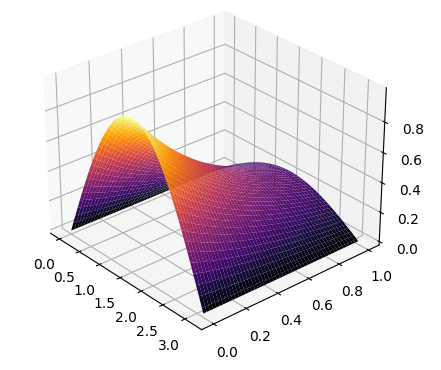
\includegraphics[width=0.5\linewidth]{ 2.png}}
            \label{ris:image}
        \end{figure}\\

        Изменение ошибки в зависимости от размера шага по пространству из 
        $$\frac{\pi}{100},\frac{\pi}{1000}~и~\frac{\pi}{10000}:$$
        \begin{figure}[h]
            \center{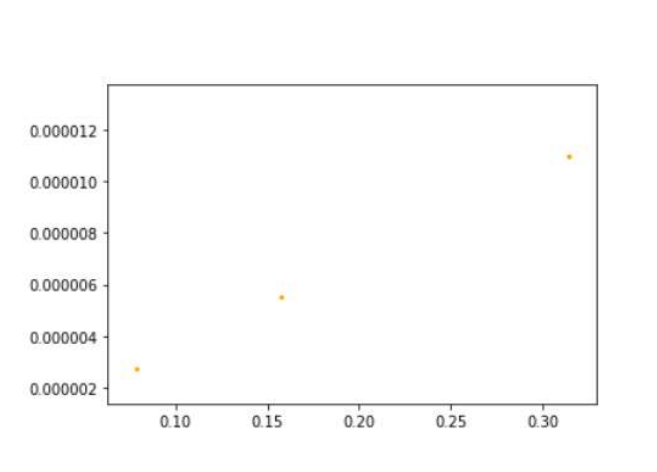
\includegraphics[width=0.5\linewidth]{ 3.png}}
            \label{ris:image}
        \end{figure}\\
        \newpage
        Явный метод:

        \begin{figure}[h]
            \center{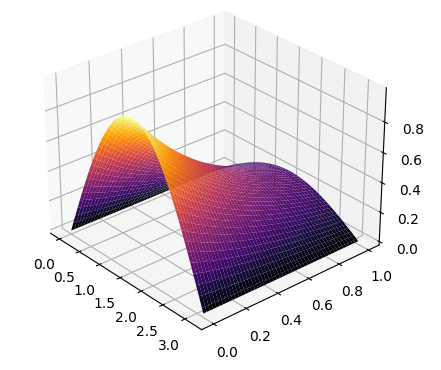
\includegraphics[width=0.5\linewidth]{ 2.png}}
            \label{ris:image}
        \end{figure}\\

        Изменение ошибки в зависимости от размера шага по пространству из 
        $$\frac{\pi}{100},\frac{\pi}{1000}~и~\frac{\pi}{10000}:$$
        \begin{figure}[h]
            \center{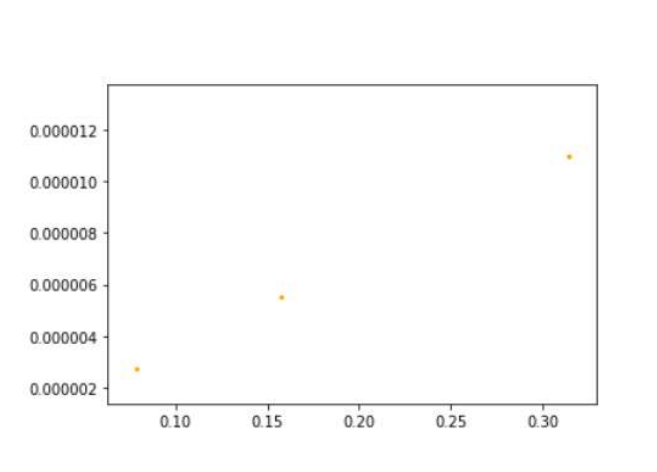
\includegraphics[width=0.5\linewidth]{ 3.png}}
            \label{ris:image}
        \end{figure}\\
        \newpage
        
        \item \textbf{Вывод:}\\
        Были реализованы два численных метода на Си для решения задачи 
        гиперболического типа.
        \\Первый – Явный метод. Он использует в правой части значения только с 
        предыдущего временного слоя,  и получает явной выражения для решения на
        новом временном слое.
        \\Второй – Неявный метод. Использует в правой части значения с текущего 
        слоя, что приводит к решению СЛАУ с помощью метода прогонки.
        \\Оба метода дали хорошую сходимость. Ошибка решений падает с уменьшением 
        размеров шагов по времени и пространству. 
        \\Были построены графики решений и ошибок по сравнению с аналитическим 
        решением. 
        
    \end{enumerate}
\end{document}